% !TeX encoding=utf8
% !TeX spellcheck = en-US

\chapter{Related work}

The main work of the project is to find different approaches for visualisation of combinatorial maps, and using these techniques to build a tool for helping more people learn about the structure. From the previous content we knew the details and application of the combinatorial maps. This section is focus on the methods for drawing the structure.

\section{Corners based method}

Dainis Zeps and Paulis Kikusts \cite{zeps2012draw} came up with the idea in 2012. They introduced a new concept called corners replacing the half-edges in combinatorial maps. Corners are formed by two neighboring oriented edges around vertices, namely, incoming head and outgoing tale. The combinatorial map consists of a pair of  permutations \((R_V,R_F)\) with corners, in which \(R_V\) and \(R_F\) are vertices rotations and faces rotations. See \cref{fig:figures:corner} the faces rotations and vertices rotations fixed from right to left. Consequently, we get \(R_V=(1\,2\,3)(4\,5\,6)(7\,8)(9\,10\,11\,12)(13\,14)\), \(R_F=(1\,11\,13)(2\,4\,10)(3\,14\,12\,8\,6)(5\,7\,9)\) , and two edges rotations \(R_{E1}=(1\,14)(2\,11)(3\,4)(5\,10)(6\,7)(8\,9)(12\,13)\) or \\\(R_{E2}=(1\,10)(2\,6)(3\,13)(4\,9)(5\,8)(7\,12)(11\,14)\).

\begin{figure}[htb]
    \centering
    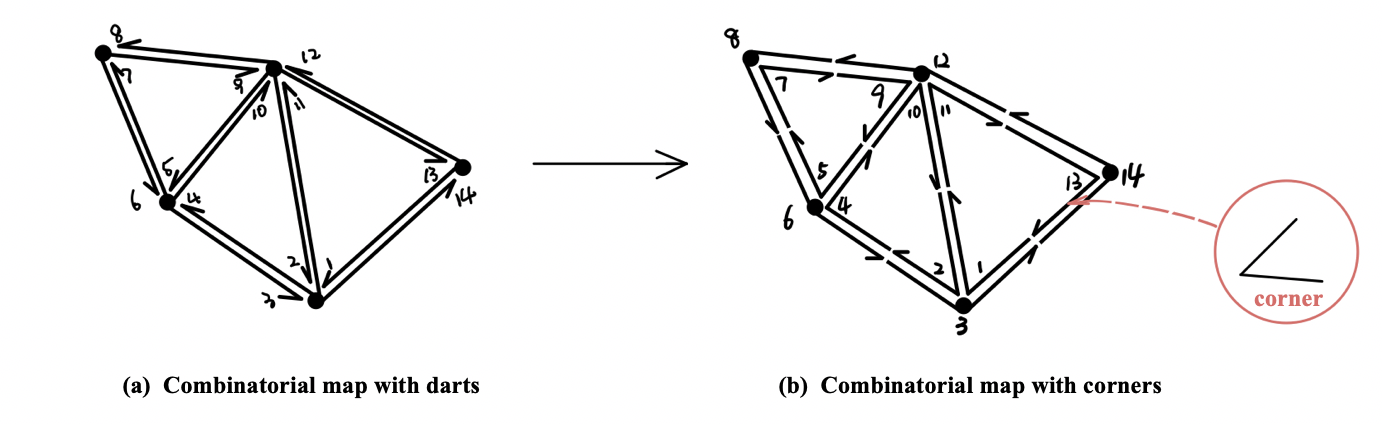
\includegraphics[width=0.8\textwidth]{../../image/corner.png}
    \caption{Combinatorial maps with corners.}
    \label{fig:figures:corner}
  \end{figure}

  Knot in maps shows the connection of corners which responses to the edges structure.Combinatorial maps involve in the partially normalised knots whose restriction is that all edges follow the same order, i.e., the less valued corners should come first, or reversely. There are three types of rotations in the combinatorial maps, so that they can be abstracted as tripe of adjacencies of corners as the image shows. The green label is vertex’s vertex, the red labeled face vertex and the blue means edge face. Uniting each labeled vertex the corresponding adjacencies can be achieved. The knot occurs into the edge adjacency or r-adjacency. At the end, through fix knots of maps and drawing the rotations via corners, the whole maps could be settled.

    \begin{figure}[htb]
      \centering
      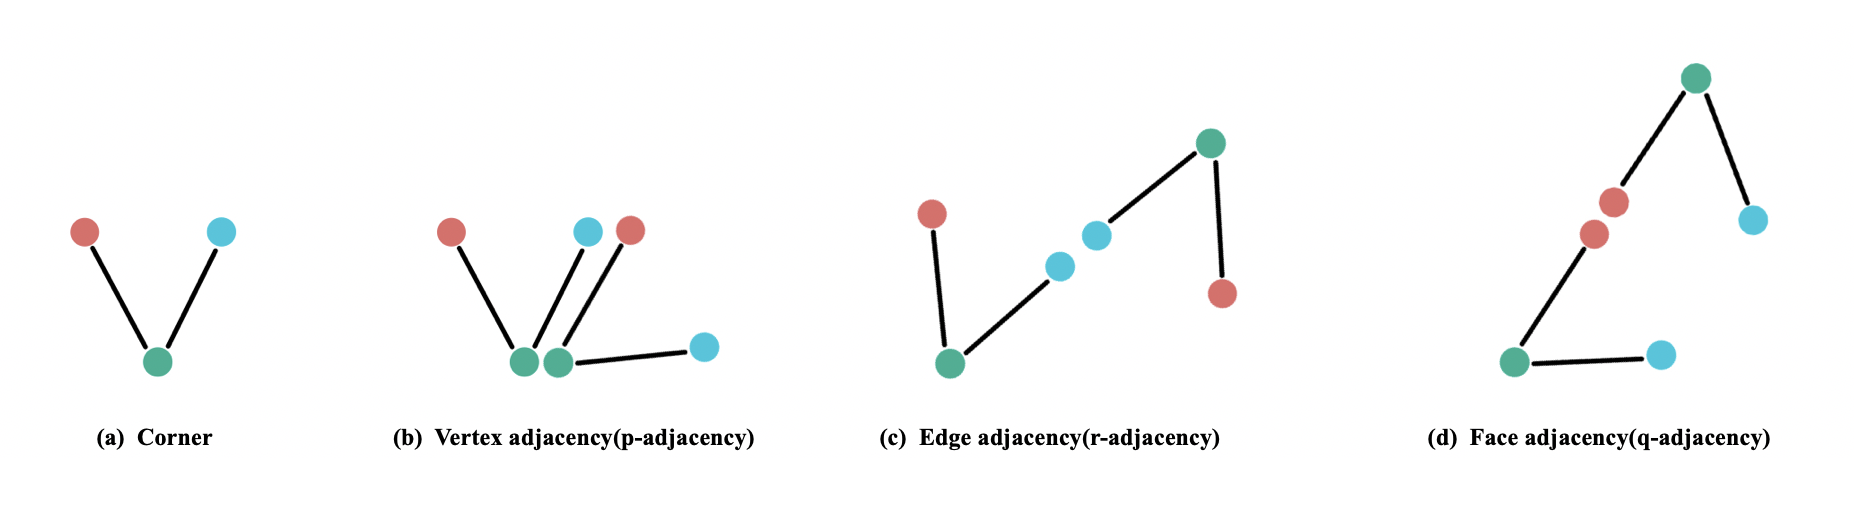
\includegraphics[width=0.8\textwidth]{../../image/adjacencies.png}
      \caption{Three adjacencies}
      \label{fig:figures:adjacencies}
    \end{figure}

In a word, this method is using the concept of corner to represent the rotations of each components. On the one hand, it produces a new angle to describe the combinatorial maps and drawing them. On the other hand, it makes the orientations constrain more clearly and directly which saves a lot of time to fix the ordered edges. 

\section{Vertices based method}

For the previous method, the authors did not discuss the layout of knots or the corners, and they did not switch the process to a useful algorithm, which confuses people who want to use the method. To explore deeply for drawing the whole combinatorial map automatically on a certain canvas, we need to pay more attention on the layout of it. There are many algorithms concern about drawing planar graphs, for example, force-directed drawing algorithms summarised by Stephen G. Kobourov \cite{kobourovg}. This algorithms provide the details of vertices layout to avoid the cross. The algorithm simulates the celestial mechanics, each vertex is seen as a star which has repulsive force and attractive force with others. Therefore, the distance between vertices depends on those forces.

An idea\cite{tingyu2019drawer} for visualisation had been came up following the classical structure of combinatorial maps and the force-directed drawing algorithm. The steps as below:

\begin{itemize}
    \item[a)] Using force-directed algorithm sets the vertices.
    \item[b)] Since the pair of darts or edges is the connection between two vertices, some darts could be settled after knowing the position of the vertices.
    \item[c)] For placing the remaining darts according to the order around the vertices, we need find a base line and calculate the existed angles between base line and other darts for each vertex, and then put the rest darts by dividing the angles. Here are the details:
    \begin{itemize} 
        \item The base line is the first dart appeared in the vertex.
        \item The equation \(angle=atan2(v1.y,v1.x)-atan2(v2.y,v2.x)\) is to calculate the angle, if the result less than 0, it needs to return \(angle=angle+2*\pi\) . The \(v1\) and \(v2\) in equation mean the direction vectors about darts.
        \item After knowing the rotating angle for a new dart, it can be places with the formula \(d.x=v1.x*cos(angle_d)+v1.y*sin(angle_d)+v.x\) and \(d.y=-v1.x*sin(angle_d)+v1.y*cos(angle_d)+v.y\) where \(d\) is the new dart and \(v\) is the vertex.
        \item Note that the orientation of darts around the vertices is anti-clockwise.
    \end{itemize}
    \item[d)] Finally, connecting darts goes by the permutation of darts. 
\end{itemize}

\begin{figure}[htb]
    \centering
    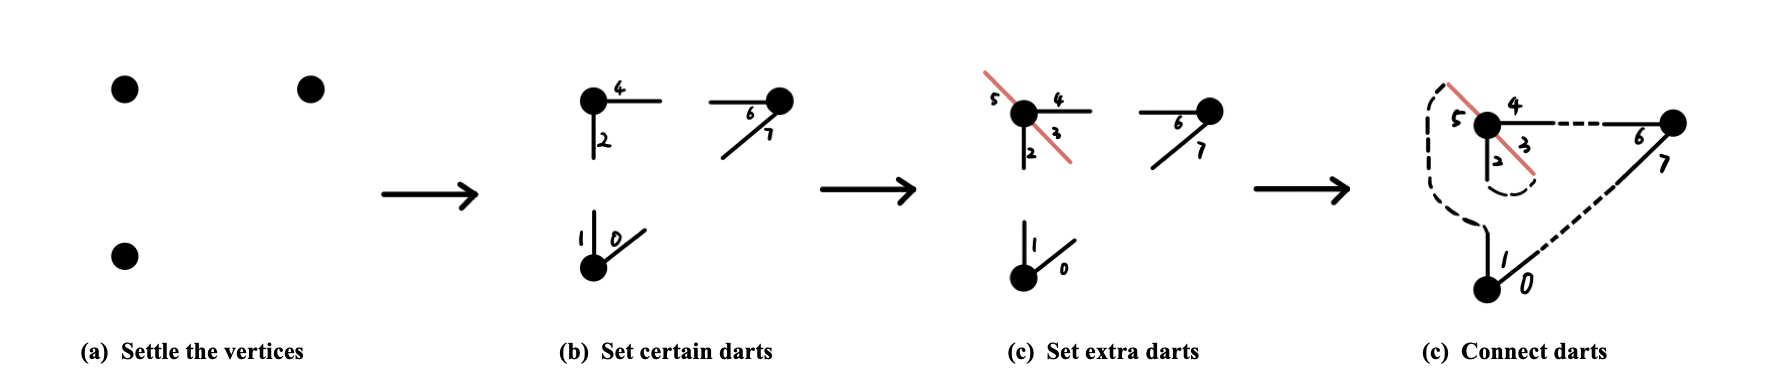
\includegraphics[width=0.8\textwidth]{../../image/firstmethod.png}
    \caption{Process of vertices based method.}
    \label{fig:figures:firstmethod}
  \end{figure}

\newpage
This method considers the whole process of drawing a map, however, it is not quite stable and have high time complexity. Its results are variant each time for the same maps, and the force-directed algorithm is the reason why this situation occurs. The \cref{fig:figures:frvertices} shows the possible vertices positions for a map produced by the algorithm. This will produce different images for the same structure, which might confuse the users.

\begin{figure}[htb]
    \centering
    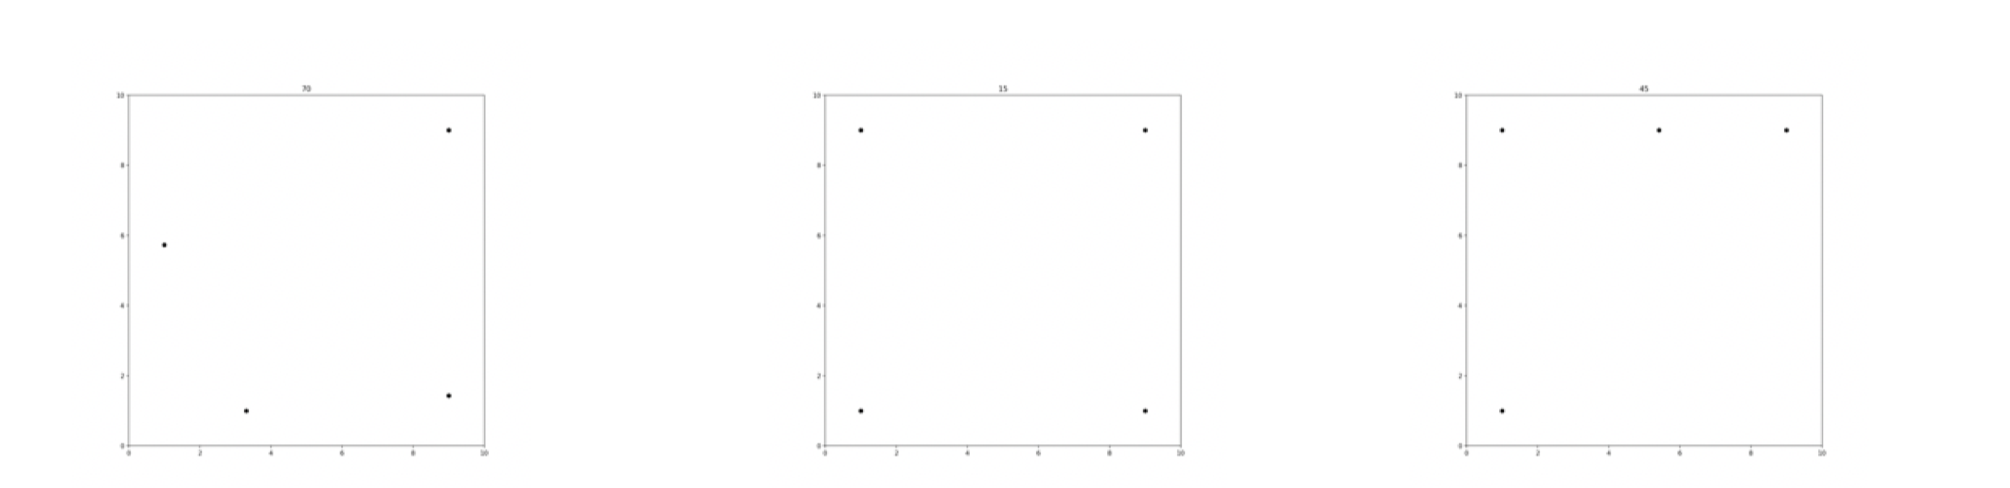
\includegraphics[width=0.8\textwidth]{../../image/frvertices.png}
    \caption{The different consequence of force-directed algorithm for a map.}
    \label{fig:figures:frvertices}
  \end{figure}